\documentclass[11pt,oneside]{book}

\usepackage[T1]{fontenc}
\usepackage[utf8]{inputenc}
\usepackage{lmodern}
\usepackage[margin=1.15in]{geometry}
\usepackage{microtype}
\usepackage{xcolor}
\usepackage{graphicx}
\usepackage{amsmath,amssymb,mathtools}
\usepackage{booktabs}
\usepackage{enumitem}
\usepackage{listings}
\usepackage[numbers,sort&compress]{natbib}
\usepackage{imakeidx}
\usepackage{tikz}
\usetikzlibrary{arrows.meta,automata,positioning,shapes.geometric}
\usepackage{pgfplots}
\pgfplotsset{compat=1.18}
\usepackage[hidelinks]{hyperref}
\usepackage[nameinlink,noabbrev]{cleveref}

\hypersetup{
  pdftitle={Grammar-based Formal Methods Vibecoding},
  pdfauthor={The LeanFM Project and ChatGPT}
}

\makeindex[intoc,title=Index]

\definecolor{leanblue}{RGB}{40,74,120}
\definecolor{leangreen}{RGB}{35,110,70}
\definecolor{leangray}{RGB}{90,90,90}
\lstdefinelanguage{Lean}{
  morekeywords={abbrev,def,deriving,inductive,namespace,structure,theorem,where,
    match,with,if,then,else,let,in,fun,forall,exists,Type,Nat,String,Bool,List},
  sensitive=true,
  morecomment=[l]{--},
  morecomment=[s]{/-}{-/},
  morestring=[b]"
}
\lstset{
  language=Lean,
  basicstyle=\ttfamily\small,
  keywordstyle=\color{leanblue}\bfseries,
  commentstyle=\color{leangreen},
  stringstyle=\color{leangray},
  columns=fullflexible,
  keepspaces=true,
  frame=single,
  breaklines=true,
  showstringspaces=false
}

\begin{document}
\pagenumbering{gobble}
\begin{titlepage}
\begin{tikzpicture}[remember picture,overlay]
  \node at (current page.center)
    {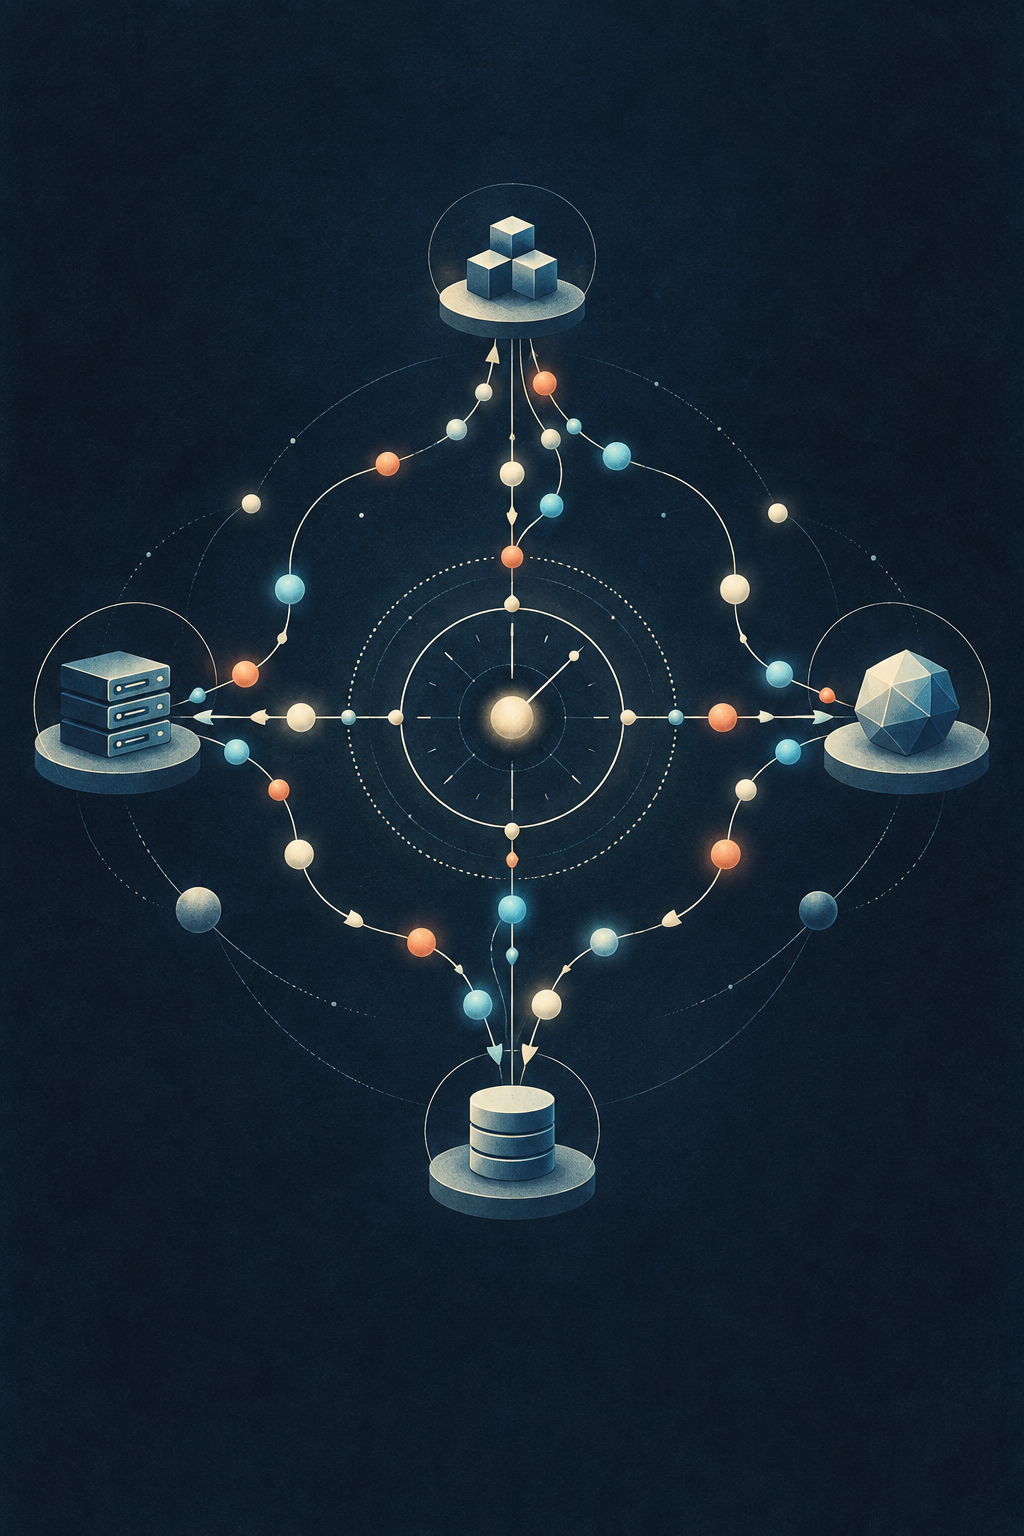
\includegraphics[width=\paperwidth,height=\paperheight]{assets/grammar-events-cover.png}};
  \fill[black,opacity=.34]
    (current page.north west) rectangle ([yshift=-4.2cm]current page.north east);
  \fill[black,opacity=.30]
    ([yshift=2.25cm]current page.south west) rectangle (current page.south east);
  \node[anchor=north west,text width=.82\paperwidth,align=left]
    at ([xshift=1.35cm,yshift=-1.25cm]current page.north west)
    {\color{white}\fontsize{31}{35}\selectfont\bfseries
      Grammar-based\\Formal Methods\\Vibecoding};
  \node[anchor=south west,text width=.78\paperwidth,align=left]
    at ([xshift=1.4cm,yshift=1.05cm]current page.south west)
    {\color{white}\Large The LeanFM Project and ChatGPT\\[.35em]
     \normalsize Working draft---\today};
\end{tikzpicture}
\end{titlepage}
\frontmatter

\chapter*{Preface}
\addcontentsline{toc}{chapter}{Preface}
Formal methods should be the easy way to build software. This book develops that
claim into a practical method: describe externally meaningful behaviour as a
parameterised, multiparty grammar; interpret its sentences as event traces; state
temporal requirements in CTL; and render the whole specification as ordinary Lean.
The specification says what participants may observe, not how an implementation
stores every intermediate detail.

This is a working book and an executable design notebook. Definitions will migrate
into a stable Lean library; systems built with the library should consist mostly of
domain types, grammar productions, and theorems about expected behaviour.
The evolving implementation, examples, and book sources are maintained in the
LeanFM repository \citep{leanfmrepo}.

\tableofcontents

\mainmatter
\part{The Grammar-Based Method}
\chapter{Formal Methods as the Default Path}
\label{ch:vision}

\index{formal methods}
Formal methods are usually presented as an extra stage: first build a system, then
translate a simplified version into a model, and finally ask a specialist tool a
few questions. That workflow taxes correctness. The model drifts, the difficult
translation is postponed, and proofs concern yesterday's architecture.

Our aim is the reverse. The shortest path to a running service should pass through
an executable behavioural specification. Writing the specification should remove
work: it supplies message types, scenario tests, model-checking input,
documentation, and the skeleton of the service itself. Going without it should be
the inconvenient choice.

\section{Behaviour before machinery}

The primary object is a set of permitted, visible histories. An implementation may
use threads, actors, queues, databases, caches, or continuations. Those decisions
matter operationally, but they are not automatically part of the contract.
Promoting all internal state into the model creates a product state space whose
size grows exponentially with independently varying components. Worse, it makes
the specification brittle under harmless refactoring.

We therefore begin with \emph{behaviour}: who communicated with whom, what kind of
event occurred, what information it carried, and what causal history it extends.
Internal state enters only when it changes an observable promise.

\section{Three ingredients}

The method combines three traditions.

\begin{enumerate}[label=\arabic*.]
  \item Language theory gives compact generative descriptions of legal histories.
        Regular and context-free grammars provide the approachable starting point.
        Dana Richards and Henry Hamburger, the author's college professors, are
        cited in \citet{richards2017logic} as the source from which the author
        learned these methods, not as their originators. For the underlying habits of
        symbolization, validity, proof, quantification, and modal reasoning, we also
        draw on the accessible progression of \citet{gensler2017introduction}.
  \item Protocol analysis contributes explicit participants, adversarial choices,
        trace semantics, and tool-supported checking. The CSP treatment of
        \citet{ryan2001modelling}, including Steve Schneider, is cited as the source
        from which the author learned this treatment.
  \item Temporal logic turns expectations into queries over the generated
        transition system. CTL is central because it distinguishes claims about
        some possible future from claims about every possible future
        \citep{clarke1986automatic}.
\end{enumerate}

\section{A test for every abstraction}

Each abstraction in this book should answer a practical question:

\begin{quote}
Can a developer state a meaningful behaviour once, compose it with other
behaviours, check its consequences, and keep it stable while implementation details
change?
\end{quote}

If an abstraction does not improve that workflow, it does not belong in the core
library.

\chapter{Histories Made of Events}
\label{ch:events}

\index{event}
\index{trace}
Every execution is represented by an event sequence. A deliberately small common
envelope makes histories comparable across protocols:

\begin{lstlisting}
structure Event (Actor Session Task Kind Payload : Type) where
  timeAt  : ClockTimestamp
  id      : String
  priorIds : List String
  session : Session
  task    : Task
  from    : Actor
  to      : Actor
  kind    : Kind
  payload : Payload

abbrev Trace (Actor Session Task Kind Payload : Type) :=
  List (Event Actor Session Task Kind Payload)
\end{lstlisting}

The fields have different jobs. \texttt{id} identifies a visible fact;
\texttt{priorIds} records zero or more immediate causal claims; \texttt{from} and
\texttt{to} name the parties; \texttt{(session, task)} correlates independently
progressing conversations; and \texttt{kind} supplies a stable discriminator.
The payload is protocol-specific and carries the parameters that flow from one
production to the next. \texttt{timeAt} is sampled from the model's shared monotonic
clock. Its differences measure elapsed time; it is not a civil-time date and its
origin is immaterial.

The causal links form a directed acyclic graph rather than a singly linked list.
An initial event has no prior identifiers. A fork is represented by several later
events that each name the same prior event. A join is represented by one event
whose \texttt{priorIds} names every branch on which it immediately depends.

\section{Compute everything from a fork/join event list}

Each event is one observation at one instant. Starting and completing are
different messages, so an event does not contain an interval. Durations are
derived by selecting the two boundary events and subtracting their timestamps.

\begin{lstlisting}
structure AnalysisEvent where
  id       : EventId
  priorIds : List EventId
  timeAt   : ClockTimestamp
  bytes    : ByteArray
  reveals  : List ValueRef

def elapsed (started completed : AnalysisEvent) : Duration :=
  completed.timeAt - started.timeAt
\end{lstlisting}

Consider the first order in \texttt{examples/bakery-events.jsonl}. Payment and
baking fork after the order is placed and join before the order is accepted:

\begin{center}
\small
\begin{tabular}{@{}llllrl@{}}
\toprule
Event & Immediate prior & \texttt{timeAt} & Meaning & Bytes & Reveals \\
\midrule
$e_0$ & $[]$ & $258726$ & order placed & 85 & order \\
$e_1$ & $[e_0]$ & $258921$ & payment requested & 71 & price \\
$e_2$ & $[e_0]$ & $259194$ & bake requested & 73 & product \\
$e_3$ & $[e_1]$ & $262219$ & payment authorized & 49 & authorization \\
$e_4$ & $[e_2]$ & $2055947$ & bake completed & 55 & completion \\
$e_5$ & $[e_3,e_4]$ & $2056288$ & order accepted & 57 & outcome \\
$e_6$ & $[e_5]$ & $2056291$ & delivery requested & 54 & delivery \\
$e_7$ & $[e_6]$ & $2283253$ & courier assigned & 40 & courier \\
$e_8$ & $[e_7]$ & $6946819$ & order delivered & 65 & outcome \\
\bottomrule
\end{tabular}
\end{center}

The list order is a serialization convenient for storage. Causal order is the
transitive closure of \texttt{priorIds}. Both $e_1$ and $e_2$ cite $e_0$, so they
fork. Event $e_5$ cites both $e_3$ and $e_4$, so it joins the branches. The
following quantities are folds or graph queries over this one list:

\begin{align*}
  \operatorname{paymentTime}(e_1,e_3) &= e_3.timeAt-e_1.timeAt = 3298,\\
  \operatorname{latency}(e_0,e_8) &= e_8.timeAt-e_0.timeAt = 6688093,\\
  \operatorname{wireBytes} &= 85+71+73+49+55+57+54+40+65 = 549.
\end{align*}

Two events are causally concurrent when neither is an ancestor of the other:

\begin{lstlisting}
def concurrent (events : List AnalysisEvent) (a b : EventId) : Bool :=
  !reachable events a b && !reachable events b a
\end{lstlisting}

The maximum concurrency permitted by the trace is the width of this partial
order: the size of its largest antichain. Here $\{e_1,e_2\}$ is an antichain, as
is $\{e_3,e_4\}$, and no three events are pairwise concurrent. Thus the maximal
causal concurrency is two. A timestamped point event has no active interval;
runtime concurrency requires separate start and completion messages. This is stronger than counting
adjacent list elements and different from measuring average runtime concurrency.

Timestamps and causal links also give elapsed time along a selected path:

\begin{lstlisting}
edgeTime(prior, event) := event.timeAt - prior.timeAt
elapsed(started, completed) := completed.timeAt - started.timeAt
\end{lstlisting}

The critical path is $e_0,e_2,e_4,e_5,e_6,e_7,e_8$, with elapsed time 6,688,093 ms.
The payment branch finishes at tick 262,219 and has 1,793,728 ms of slack before the join.
Queue occupancy, queued
bytes, active \texttt{(session,task)} keys, and memory pressure are computed by
adding enqueue/dequeue events to the same alphabet and folding them in clock
order.

The entire checked-in corpus contains \BakeryOrders{} orders and
\BakeryEvents{} events. Streaming that file produces the following model inputs;
the numbers in this table are generated LaTeX macros, not independently typed
constants:

\begin{center}
\begin{tabular}{@{}lr@{}}
\toprule
Reduction over \texttt{bakery-events.jsonl} & Observed value \\
\midrule
payment authorized / orders & \BakeryPaymentRatio \\
bake completed / orders & \BakeryBakeRatio \\
order accepted / orders & \BakeryAcceptRatio \\
delivered / orders & \BakeryDeliveredRatio \\
mean terminal latency & \BakeryMeanLatency{} ms \\
median terminal latency & \BakeryPFiftyLatency{} ms \\
95th-percentile terminal latency & \BakeryPNinetyFiveLatency{} ms \\
maximum simultaneously active orders & \BakeryMaxActive \\
\bottomrule
\end{tabular}
\end{center}

These ratios are suitable probability estimates for this corpus. Regeneration
with a different source stream changes the macros and therefore changes every
book example that consumes them.

Knowledge is another event reduction. For a value $v$, calculate the actors that
can derive it from initial knowledge and the bytes visible to them:

\begin{lstlisting}
def knowers (actors : List Actor) (v : ValueRef)
    (events : List AnalysisEvent) : List Actor :=
  actors.filter fun actor =>
    Derives (knowledgeFrom actor events) v
\end{lstlisting}

Encryption, signing, projection, key possession, and compromise contribute rules
to \texttt{Derives}. The primary result is the set \texttt{knowers v events}.
``Only these actors know $v$'' is a comparison between that computed set and an
allowed set, not a separate primitive called secrecy.

\section{Derived state}

A current session, an authenticated principal, or an outstanding request can often
be computed by folding the trace. Such a fact need not also exist as primitive
model state. This discipline has two benefits: evidence for a fact remains visible,
and the state representation does not multiply independently of the history that
justifies it.

Some implementations necessarily maintain private state. The model includes it
only when two executions with the same visible trace may make different future
behaviour legal. Even then, the first remedy is to expose the relevant distinction
as an event or a grammar parameter rather than copying an implementation object
graph into the specification.

\section{Time is more than a timestamp}

\index{time}
The central modelling problem is maintainable time evolution. We separate three
ideas that are often conflated:

\begin{itemize}
  \item sequence order: one visible event occurs before another;
  \item causality: an event extends or responds to another event;
  \item duration: an amount of physical or logical time elapses.
\end{itemize}

Grammar structure handles sequence, identifiers handle causal linkage, and typed
constraints handle duration. This keeps a change in timeout policy from rewriting
the protocol's entire behavioural shape.

For two events from the same \texttt{(session, task)}, elapsed time is defined when
the first event's \texttt{timeAt} value does not exceed the second's:

\begin{lstlisting}
def elapsed (start finish : Event) : Option Duration :=
  if start.session = finish.session &&
     start.task = finish.task &&
     start.timeAt <= finish.timeAt
  then some (finish.timeAt - start.timeAt)
  else none
\end{lstlisting}

Latency queries name their boundary event kinds and correlate them by
\texttt{(session, task)} before subtracting timestamps. Causality still comes
from grammar structure and \texttt{priorIds}: equal timestamps may occur, and a
timestamp alone does not establish that one event caused another.

\section{Round trip through bytes}

A generated scenario is not complete until it can cross the byte boundary in
both directions. \texttt{ScenarioEvent} in \texttt{Requirements.proto} carries
the event identity, complete \texttt{prior} list, correlation key, actors,
\texttt{timeAt}, and the selected protobuf atom. Encoding a \texttt{Scenario}
therefore produces bytes for both its causal envelope and payload. Decoding those
bytes must reconstruct the same ordered event list. The executable round-trip
check compares the decoded protobuf value with the generated value and separately
checks the reconstructed \texttt{prior} graph; loss of a fork or join fails the
build.

\chapter{A Multiparty Grammar of Behaviour}
\label{ch:grammar}

\index{grammar!multiparty}
\index{grammar!context-free}
A protocol is a language whose terminal symbols are visible events. A production
describes a legal continuation. The context-free grammar is the visual and
conceptual starting point, not a claim that every useful protocol language is
context-free.

\section{A small authoring algebra}

\begin{lstlisting}
inductive Grammar (Event : Type) where
  | empty
  | event  : Event -> Grammar Event
  | seq    : Grammar Event -> Grammar Event -> Grammar Event
  | choice : List (Grammar Event) -> Grammar Event
  | par    : Grammar Event -> Grammar Event -> Grammar Event
  | where_ : (List Event -> Bool) -> Grammar Event -> Grammar Event
\end{lstlisting}

\texttt{seq} preserves time order. \texttt{choice} exposes alternatives rather
than burying them in control flow. \texttt{par} admits interleavings while
preserving the internal order of each side. A \texttt{where\_} clause checks a
fact accumulated from the prior trace and provides the escape from context-free
structure when genuine context sensitivity is needed.

Simple finite conversations can compile to regular languages. Nested request
structure motivates context-free productions. Correlation, freshness, uniqueness,
and authorization typically require parameter flow or guarded productions.

\section{Parameters carry information}

\index{parameter flow}
A production should bind values at one event and reuse them later. Conceptually:

\begin{lstlisting}
def login (browser server provider : Actor) (state : OAuthState) : Grammar Event :=
  event (redirect server browser provider state) >>>
  event (authorize browser provider state) >>>
  callback browser server state
\end{lstlisting}

The repeated \texttt{state} is not decorative. It states the information-flow
relationship that distinguishes a matching callback from an unrelated one. Lean's
types, constructors, and ordinary function parameters are the surface language;
the fixed library supplies grammar composition and semantics.

\section{Composition without omniscience}

A participant's implementation need not know the global execution state. The
global grammar states the contract, while projection derives each participant's
view. Composition should preserve independently specified modules and make shared
events explicit. Proving useful projection and composition theorems is a core
research obligation, not an implementation footnote.

\chapter{The Scenario Authoring Language}
\label{ch:authoring-language}

\index{scenario}
\index{observable event}
This chapter proposes the first concrete surface language. It is intentionally a
small Lean DSL: ordinary \texttt{def}, function parameters, \texttt{let}, typed
values, and \texttt{do} notation provide the host language; a fixed library adds
scenario, endpoint, choice, probability, and rendering operations. The examples
are a design target. Names may change as the Lean implementation makes their
semantics precise.

\section{The smallest useful scenario}

A scenario is a named grammar fragment. Every emitted terminal is an observable
message event. Endpoint commands establish the \texttt{from} and \texttt{to}
context for the messages that follow.

\begin{lstlisting}
def requestQuote (customer shop : Actor) : Scenario :=
  scenario "request a quote" do
    let requestId <- declare RequestId "requestId"

    from_ customer
    to_ shop
    emit "quote requested" [field "requestId" requestId]

    let quoteId <- declare QuoteId "quoteId"
    let amount  <- declare Money "amount"

    from_ shop
    to_ customer
    emit "quote offered"
      [ field "requestId" requestId
      , field "quoteId" quoteId
      , field "amount" amount
      ]
\end{lstlisting}

The spelling \texttt{from\_} avoids collision with Lean syntax while remaining
visually explicit. Endpoint commands affect authoring context only; elaboration
copies both endpoints into every event. A scenario with an \texttt{emit} before
both endpoints have been established is rejected.

\subsection{Variables and assignment}

There are two kinds of assignment.

\begin{itemize}
  \item Ordinary \texttt{let x := expression} evaluates a known Lean expression.
  \item \texttt{let x <- declare T "x"} introduces a symbolic value of type
        \texttt{T}. The grammar binds it when generating or matching a trace, and
        later events may reuse it.
\end{itemize}

Variables are immutable. A later \texttt{let attempt := attempt + 1} creates a new
binding rather than mutable hidden state. Information flow is consequently visible
in the grammar's data dependencies. Equality of two occurrences of
\texttt{requestId} means they carry the same value, not merely values with the same
field name.

A value received from the environment is bound by matching an observable event:

\begin{lstlisting}
from_ customer
to_ shop
receive "quote accepted" do
  let quoteId <- take QuoteId "quoteId"
  let payment <- take PaymentToken "paymentToken"

from_ shop
to_ bank
emit "payment authorization requested"
  [field "quoteId" quoteId, field "paymentToken" payment]
\end{lstlisting}

\texttt{receive} and \texttt{emit} both denote grammar terminals; they differ only
in the viewpoint used when projecting a global scenario to executable participant
code.

\section{Vague messages first, typed alphabets later}

\index{alphabet!vague}
Early requirements should not require a finished protobuf schema. A vague message
has a stable semantic name and a list of named, typed fields. It is already precise
enough to express ordering, correlation, and temporal properties.

\begin{lstlisting}
emit "quote offered"
  [field "requestId" requestId, field "amount" amount]
\end{lstlisting}

Later, a refinement maps that terminal to a concrete alphabet:

\begin{lstlisting}
refineMessage "quote offered" with Proto.Shop.QuoteOffered where
  request_id := field "requestId"
  quote_id   := field "quoteId"
  cents      := encodeMoney (field "amount")
\end{lstlisting}

The refinement obligation is language inclusion: every concrete implementation
trace, after erasing representation details, must be admitted by the abstract
grammar. Refinement may decide serialization, retry mechanics, and internal state;
it must not invent externally visible behaviour forbidden by the requirements.

\section{One concern per scenario}

Scenarios should be small enough to read as stories and independent enough to
render separately. The quote protocol can be decomposed as follows.

\begin{lstlisting}
def quoteAccepted (customer shop : Actor) : Scenario :=
  scenario "quote accepted" do
    include (requestQuote customer shop)
    -- bind quoteId from the included scenario's exports
    use quoteId <- exported QuoteId "quoteId"
    from_ customer; to_ shop
    emit "quote accepted" [field "quoteId" quoteId]

def quoteDeclined (customer shop : Actor) : Scenario :=
  scenario "quote declined" do
    include (requestQuote customer shop)
    use quoteId <- exported QuoteId "quoteId"
    from_ customer; to_ shop
    emit "quote declined" [field "quoteId" quoteId]

def quoteOutcome (customer shop : Actor) : Scenario :=
  oneOf "customer decision"
    [ quoteAccepted customer shop
    , quoteDeclined customer shop
    ]
\end{lstlisting}

\texttt{include} is textual only in the rendered book view; semantically it is a
reference to a named nonterminal. The compiler reads all referenced scenarios,
checks exported bindings, detects cycles, and builds one grammar. Tools retain the
scenario boundary for navigation, diagrams, tests, and counterexamples.

\section{Interaction diagram: accepted quote}

The first rendering of any scenario is a sequence-style interaction diagram.
It shows observable messages and parameter flow without suggesting an internal
implementation architecture.

\begin{figure}[htbp]
\centering
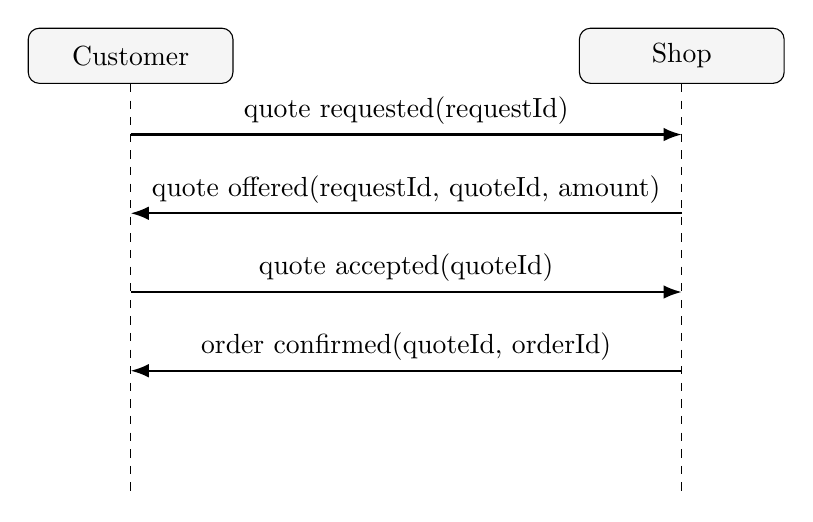
\begin{tikzpicture}[>=Latex,actor/.style={draw,rounded corners,minimum width=2.6cm,
  minimum height=.7cm,fill=black!4},message/.style={->,thick}]
  \node[actor] (customer) at (0,0) {Customer};
  \node[actor] (shop) at (7,0) {Shop};
  \draw[dashed] (customer.south) -- ++(0,-5.2);
  \draw[dashed] (shop.south) -- ++(0,-5.2);
  \draw[message] (0,-1) -- node[above,sloped]{quote requested(requestId)} (7,-1);
  \draw[message] (7,-2) -- node[above,sloped]{quote offered(requestId, quoteId, amount)} (0,-2);
  \draw[message] (0,-3) -- node[above,sloped]{quote accepted(quoteId)} (7,-3);
  \draw[message] (7,-4) -- node[above,sloped]{order confirmed(quoteId, orderId)} (0,-4);
\end{tikzpicture}
\caption{Interaction diagram derived from the accepted-quote scenario.}
\label{fig:quote-interaction}
\end{figure}

\section{Choices and unresolved probability}

\index{probability}
Nondeterminism and probability are different. \texttt{oneOf} says that multiple
behaviours are legal without claiming how often they occur. \texttt{weighted}
attaches a distribution when the abstraction has one.

\begin{lstlisting}
def paymentOutcome : Scenario :=
  oneOf "payment outcome" [paymentApproved, paymentRejected]

def estimatedPaymentOutcome : Scenario :=
  choose "estimated payment outcome"
    [ weighted (95 / 100) paymentApproved
    , weighted ( 5 / 100) paymentRejected
    ]
\end{lstlisting}

Probabilities belong to choices, not to messages. An early requirement can use
\texttt{oneOf}, a symbolic weight, or a range such as \texttt{between 0.90 0.99}.
Implementation refinement resolves those claims to a well-defined stochastic
model or to deterministic conditions. Refinement must preserve possibility even
when a current implementation assigns probability zero to a legal abstract branch;
otherwise changing operational policy would silently change the contract.

\section{Composing requirements means intersecting constraints}

\index{composition!requirement intersection}
Scenario composition builds behaviour in familiar language-theoretic ways:

\begin{center}
\begin{tabular}{@{}lll@{}}
\toprule
Operator & Language operation & Purpose \\
\midrule
\texttt{then a b} & concatenation & $a$ happens before $b$ \\
\texttt{oneOf [a,b]} & union & either story is legal \\
\texttt{together a b} & shuffle/interleaving & independent concurrent stories \\
\texttt{repeat a} & closure & repeated conversation \\
\texttt{where\_ p a} & trace filtering & context-sensitive legality \\
\bottomrule
\end{tabular}
\end{center}

Combining requirements is subtler. A requirement usually does not add another
message sequence; it removes histories that violate a concern. Therefore
\texttt{requireAll} denotes intersection of accepted trace sets.

\begin{lstlisting}
def quoteSystem : SystemSpec :=
  generatedBy quoteOutcome
  |> requireAll
      [ correlate "offered quote matches request"
          (sameField "requestId")
      , forbid "confirmation without acceptance"
          (event "order confirmed" && notPreviously "quote accepted")
      , ctl "every accepted quote is answered"
          (AG (accepted --> AF (confirmed || rejected)))
      , timing "answer within service objective"
          (accepted --> within 2.seconds (confirmed || rejected))
      ]
\end{lstlisting}

This distinction prevents an important category error: union and concatenation
assemble possible stories; intersection layers independent obligations over those
stories. A system is consistent only if the intersection remains nonempty. When it
is empty, tooling should return a minimal conflicting set of requirements and the
shortest available counterexample prefix.

\section{State-machine rendering}

The same scenario grammar can be rendered as a state machine. States are grammar
residuals---the legal continuations after a trace prefix---rather than snapshots of
private implementation memory.

\begin{figure}[htbp]
\centering
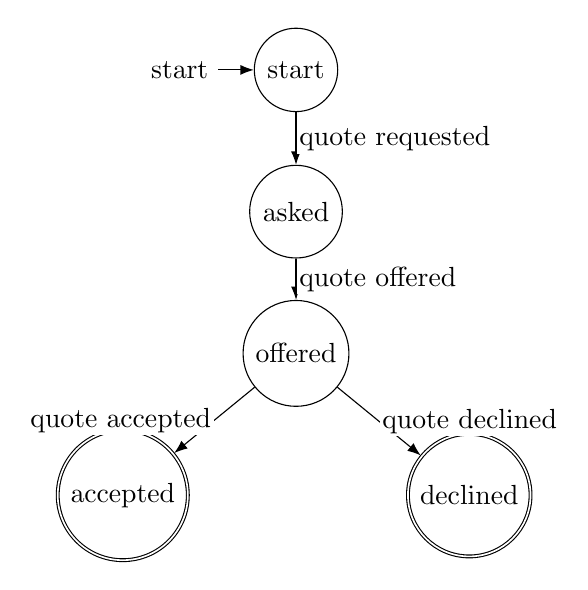
\begin{tikzpicture}[->,>=Latex,node distance=1.8cm,on grid,
  every state/.style={draw,minimum size=1.05cm}]
  \node[state,initial] (start) {start};
  \node[state] (asked) [below=of start] {asked};
  \node[state] (offered) [below=of asked] {offered};
  \node[state,accepting] (accepted) [below left=1.8cm and 2.2cm of offered] {accepted};
  \node[state,accepting] (declined) [below right=1.8cm and 2.2cm of offered] {declined};
  \path
    (start) edge node[right,fill=white,inner sep=1pt] {quote requested} (asked)
    (asked) edge node[right,fill=white,inner sep=1pt] {quote offered} (offered)
    (offered) edge node[left,fill=white,inner sep=1pt,align=right] {quote accepted} (accepted)
    (offered) edge node[right,fill=white,inner sep=1pt,align=left] {quote declined} (declined);
\end{tikzpicture}
\caption{A state machine derived from grammar residuals.}
\label{fig:quote-state-machine}
\end{figure}

\section{Charts are declarative trace reductions}

\index{chart specification}
Charts are also specified in the Lean subset. A chart names an observable event
source, a grouping or $x$ expression, and an aggregate or $y$ expression. It does
not contain rendering code.

\begin{lstlisting}
def outcomeShare : ChartSpec :=
  pie "quote outcomes" do
    source events
    where_ (kind == "quote accepted" || kind == "quote declined")
    groupBy kind
    value count

def responseLatency : ChartSpec :=
  line "quote response latency" do
    source (correlate events by "quoteId")
    x tstamp
    y (elapsed "quote offered" "customer decision")
    series "p50" median
\end{lstlisting}

\begin{figure}[htbp]
\centering
\begin{minipage}{.43\textwidth}
\centering
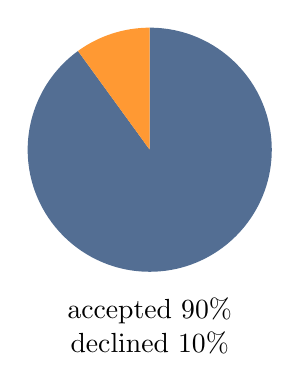
\begin{tikzpicture}
  \def\r{1.55}
  \fill[leanblue!80] (0,0) -- (90:\r) arc (90:-234:\r) -- cycle;
  \fill[orange!80] (0,0) -- (-234:\r) arc (-234:-270:\r) -- cycle;
  \node at (0,-2.05) {accepted 90\%};
  \node at (0,-2.45) {declined 10\%};
\end{tikzpicture}
\end{minipage}\hfill
\begin{minipage}{.52\textwidth}
\centering
\resizebox{.97\linewidth}{!}{%
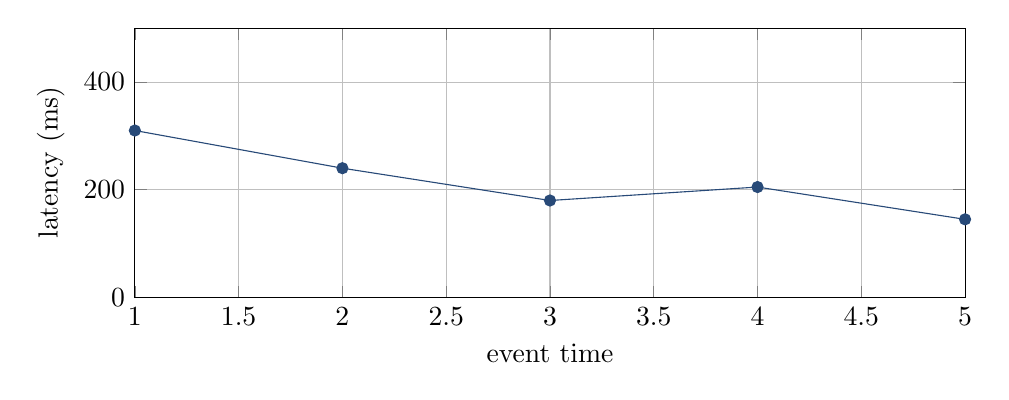
\begin{tikzpicture}
\begin{axis}[
  width=\linewidth,height=5cm,
  xlabel={event time},ylabel={latency (ms)},
  xmin=1,xmax=5,ymin=0,ymax=500,
  grid=major]
  \addplot[color=leanblue,mark=*] coordinates {(1,310) (2,240) (3,180) (4,205) (5,145)};
\end{axis}
\end{tikzpicture}
}
\end{minipage}
\caption{Example pie and line renderings from declarative chart specifications.}
\label{fig:charts}
\end{figure}

Interaction diagrams, state machines, and charts are projections of the same typed
scenario and event definitions. Keeping them derived prevents a diagram from
becoming a second, drifting specification.

\chapter{Worked Example: OAuth Authorization Code Flow}
\label{ch:oauth-example}

\index{OAuth}
This chapter is a behavioural sketch inspired by the OAuth authorization-code
flow. It is not a replacement for the OAuth specification and deliberately begins
above HTTP and protobuf. Its purpose is to exercise scenario decomposition,
parameter flow, visible evidence, alternatives, requirements, and rendering.

\section{Actors, values, and observable events}

The example has four participants: a person using a browser, an application, an
authorization service, and a resource service. The browser is modelled separately
from the person because redirects are observable messages between software
participants.

\begin{lstlisting}
inductive Actor where
  | user | browser | app | authorizationServer | resourceServer

opaque State       : Type
opaque AuthCode    : Type
opaque AccessToken : Type
opaque Resource    : Type
opaque Profile     : Type
opaque Password    : Type
opaque Bytes       : Type
\end{lstlisting}

Every terminal elaborates to the common event envelope. For example, the vague
message ``authorization redirected'' becomes conceptually:

\begin{lstlisting}
{ tstamp := t2, id := e2, priorIds := [e1]
, from := Actor.app, to := Actor.browser
, kind := "authorization redirected"
, fields := [field "state" state, field "redirectUri" callback]
}
\end{lstlisting}

\section{Scenario 1: begin authorization}

Before the redirect returns, the authorization service may authenticate the person.
OAuth does not prescribe the authentication mechanism; we include a password branch
to exercise secret input without pretending that the password is an OAuth protocol
parameter.

\begin{lstlisting}
def authenticateAtAuthorizationServer (password : Password) : Scenario :=
  scenario "authenticate resource owner" do
    from_ .browser
    to_ .authorizationServer
    emitBytes "credentials submitted"
      (protectFor .authorizationServer
        (encode [secretField "password" password]))

    from_ .authorizationServer
    to_ .browser
    oneOf "authentication result"
      [ emitBytes "authentication accepted" (encode [tag 1])
      , emitBytes "authentication rejected" (encode [tag 0])
      ]
\end{lstlisting}

The wire bytes are specified even though the transport is not. The abstract
\texttt{protectFor} constructor promises confidentiality to the named endpoint. A
later refinement may realize that promise with TLS, message-level encryption, or a
local trusted channel. Merely placing the password inside a field would not support
a secrecy theorem: a network observer would then derive it from the bytes.

\begin{lstlisting}
def beginAuthorization (resource : Resource) : Scenario :=
  scenario "begin authorization" do
    let state <- declare State "state"
    let callback := Uri.https "app.example" "/oauth/callback"

    from_ .user
    to_ .browser
    emit "resource requested" [field "resource" resource]

    from_ .browser
    to_ .app
    emit "application request" [field "resource" resource]

    from_ .app
    to_ .browser
    emit "authorization redirected"
      [field "state" state, field "redirectUri" callback]

    from_ .browser
    to_ .authorizationServer
    emit "authorization requested"
      [field "state" state, field "redirectUri" callback]

    export "state" state
    export "resource" resource
\end{lstlisting}

This scenario establishes the correlation value \texttt{state}. Nothing here says
how the application stores it. The contract only requires later observable
messages to carry the corresponding value.

\section{Scenario 2: grant or deny}

\begin{lstlisting}
def authorizationGranted : Scenario :=
  scenario "authorization granted" do
    use state <- imported State "state"
    let code <- declare AuthCode "code"

    from_ .authorizationServer
    to_ .browser
    emit "authorization code returned"
      [field "state" state, field "code" code]

    from_ .browser
    to_ .app
    emit "authorization callback"
      [field "state" state, field "code" code]
    export "code" code

def authorizationDenied : Scenario :=
  scenario "authorization denied" do
    use state <- imported State "state"
    from_ .authorizationServer
    to_ .browser
    emit "authorization error returned"
      [field "state" state, field "reason" "access_denied"]
    from_ .browser
    to_ .app
    emit "authorization error callback"
      [field "state" state, field "reason" "access_denied"]

def authorizationDecision : Scenario :=
  oneOf "authorization decision"
    [authorizationGranted, authorizationDenied]
\end{lstlisting}

The abstract contract makes both decisions possible. A product model may later
attach an estimated or measured probability distribution without changing the set
of legal traces.

\section{Scenario 3: exchange the code and use the token}

\begin{lstlisting}
def exchangeAndFetch : Scenario :=
  scenario "exchange code and fetch resource" do
    use code     <- imported AuthCode "code"
    use resource <- imported Resource "resource"
    let token    <- declare AccessToken "accessToken"
    let profile  <- declare Profile "profile"

    from_ .app
    to_ .authorizationServer
    emit "token requested" [field "code" code]

    from_ .authorizationServer
    to_ .app
    emit "access token issued" [field "accessToken" token]

    from_ .app
    to_ .resourceServer
    emit "protected resource requested"
      [field "accessToken" token, field "resource" resource]

    from_ .resourceServer
    to_ .app
    emit "protected resource returned"
      [field "resource" resource, field "profile" profile]

    from_ .app
    to_ .browser
    emit "application response" [field "profile" profile]
\end{lstlisting}

The token itself is visible only at the endpoints where the abstract protocol says
it is transmitted. The grammar makes no claim about the authorization server's
database schema or the application's session representation.

\section{Reading the scenarios together}

\begin{lstlisting}
def oauthAuthorization (resource : Resource) (password : Password) : Scenario :=
  scenario "OAuth authorization code flow" do
    include (beginAuthorization resource)
    include (authenticateAtAuthorizationServer password)
    include authorizationDecision
    after authorizationGranted include exchangeAndFetch

def oauthSystem (resource : Resource) (password : Password) : SystemSpec :=
  generatedBy (oauthAuthorization resource password)
  |> requireAll oauthRequirements
\end{lstlisting}

The \texttt{after} line is a guarded nonterminal reference. The denial branch ends
without exchanging a code. All scenario sources are read into one grammar, but
their names and boundaries remain available to render and test independently.

\section{Interaction diagrams by scenario}

\begin{figure}[p]
\centering
\resizebox{\textwidth}{!}{\OAuthInteractionDiagram{black}{white}{black!4}}
\caption{OAuth interaction view. The frames bracket the two alternatives after
the common authorization prefix; only the granted branch continues to token
exchange and resource access.}
\label{fig:oauth-interaction}
\end{figure}

\section{Requirements as observable constraints}

\begin{lstlisting}
def oauthRequirements : List Requirement :=
  [ require "callback state matches request"
      (on "authorization callback" (previouslySame "state"
        "authorization requested"))

  , forbid "code exchange after denial"
      (previously "authorization denied" && event "token requested")

  , require "issued token came from a code"
      (on "access token issued" (previouslySame "code" "token requested"))

  , ctl "every decision reaches the application"
      (AG (decisionAtAuthorizationServer --> AF callbackAtApplication))

  , ctl "a protected result is never returned without a token request"
      (AG (resourceReturned --> previously tokenRequested))
  ]
\end{lstlisting}

\subsection{Password secrecy}

\index{password secrecy}
Observable events are not the same as universally readable plaintext. Every actor
may observe that credential bytes were sent; only actors within the trusted
user-agent boundary and authorization service may derive the password value. The
theorem must name both the observer and its assumptions.

\begin{lstlisting}
theorem oauth_password_secret
    (trace : Trace WireEvent)
    (accepted : (oauthSystem resource password).Accepts trace)
    (initial : InitiallyKnown password [.browser, .authorizationServer])
    (honest : Uncompromised [.browser, .authorizationServer])
    (protection : PerfectProtection protectFor) :
    not (Derives (knowledgeOf .networkAttacker trace) (secret password)) := by
  exact protectedFieldNotDerivable accepted initial honest protection
\end{lstlisting}

This statement deliberately permits the trusted browser boundary and authorization
service to know the password. A theorem claiming secrecy from the browser would be
false for a password typed into that browser. If the desired boundary is narrower,
the actor model must represent a trusted credential component separately.

The theorem is also conditional. A compromised endpoint, logging side channel, or
failed concrete protection refinement invalidates an assumption rather than being
hidden by the grammar.

\subsection{Byte-level refinement without choosing a transport}

Every vague OAuth message can be assigned a canonical byte term before HTTP or
protobuf is chosen:

\begin{lstlisting}
refineMessage "authorization requested" where
  term := tuple
    [ tagBytes 0x01
    , namedBytes "state" (encode state)
    , namedBytes "redirectUri" (encode callback)
    ]
  bytes := encodeCanonical term

refineMessage "token requested" where
  term := tuple [tagBytes 0x02, namedBytes "code" (encode code)]
  bytes := encodeCanonical term
\end{lstlisting}

This fixes framing, tags, and value relationships at an abstract byte-algebra level.
A subsequent HTTP mapping might put those bytes into form fields; a protobuf mapping
might use numbered fields. Either concrete alphabet must prove that decoding and
re-encoding preserve the abstract terminal and its parameter bindings.

The use of \texttt{previously} is deliberately a trace predicate in this first
version. It can later receive dedicated past-time syntax without changing the event
model.

\section{Probabilities and charts}

An operational model may refine the decision and exchange outcomes:

\begin{lstlisting}
def measuredAuthorizationDecision : Scenario :=
  choose "authorization decision"
    [ weighted (87 / 100) authorizationGranted
    , weighted (13 / 100) authorizationDenied ]

def oauthCharts : List ChartSpec :=
  [ pie "authorization outcomes" do
      source events; groupBy terminalOutcome; value count
  , line "end-to-end authorization latency" do
      source (correlate events by "state")
      x tstamp; y (elapsed "authorization requested" "application response")
  ]
\end{lstlisting}

The percentages are model inputs or measurements, not truths inferred from the
grammar. The grammar continues to define which behaviours are possible; the
probabilistic refinement says how mass is distributed over them.

\section{Residual state machine}

\begin{figure}[htbp]
\centering
\resizebox{\textwidth}{!}{%
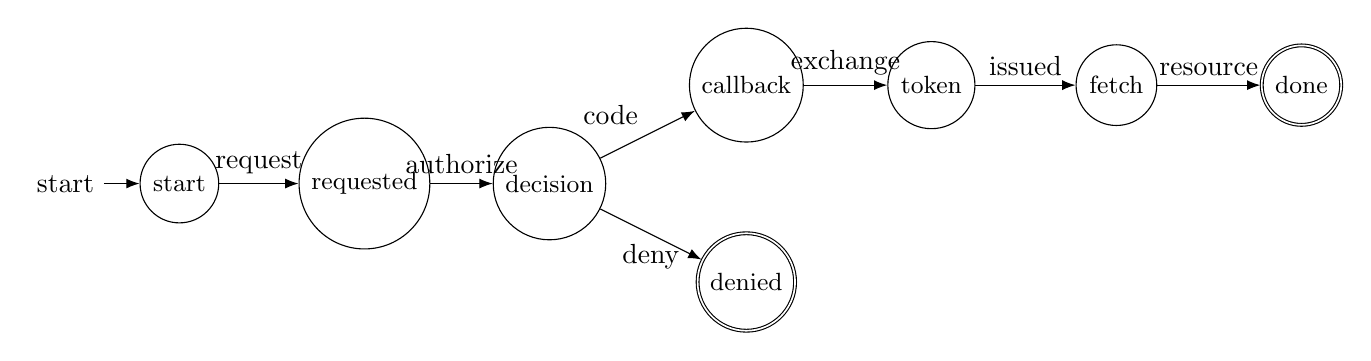
\begin{tikzpicture}[->,>=Latex,node distance=2.35cm,on grid,auto,
  every state/.style={draw,minimum size=.9cm,font=\small}]
  \node[state,initial] (start) {start};
  \node[state] (requested) [right=of start] {requested};
  \node[state] (decision) [right=of requested] {decision};
  \node[state] (callback) [above right=1.25cm and 2.5cm of decision] {callback};
  \node[state,accepting] (denied) [below right=1.25cm and 2.5cm of decision] {denied};
  \node[state] (token) [right=of callback] {token};
  \node[state] (fetch) [right=of token] {fetch};
  \node[state,accepting] (done) [right=of fetch] {done};
  \path
    (start) edge node {request} (requested)
    (requested) edge node {authorize} (decision)
    (decision) edge node {code} (callback)
    (decision) edge node[below] {deny} (denied)
    (callback) edge node {exchange} (token)
    (token) edge node {issued} (fetch)
    (fetch) edge node {resource} (done);
\end{tikzpicture}}
\caption{OAuth state machine derived from legal grammar continuations.}
\label{fig:oauth-state-machine}
\end{figure}

This automaton is intentionally behavioural. It does not contain browser cookies,
database rows, server threads, or cryptographic library state. Those details may be
essential to an implementation proof, but they are refinements of this contract,
not the contract itself.

\chapter{CTL over Generated Futures}
\label{ch:ctl}

\index{CTL}
\index{temporal logic}
A grammar generates a branching transition system. CTL speaks directly about that
branching: path quantifiers distinguish \emph{there exists a future} from
\emph{every future}, while temporal operators distinguish the next state,
eventuality, invariance, and until.

\begin{center}
\begin{tabular}{@{}lll@{}}
\toprule
Formula & Reading & Typical use \\
\midrule
$EF\,p$ & some future can reach $p$ & possibility / witness \\
$AF\,p$ & every future eventually reaches $p$ & termination / response \\
$EG\,p$ & some path preserves $p$ forever & viable invariant path \\
$AG\,p$ & every reachable state satisfies $p$ & safety invariant \\
$(p\ AU\ q)$ & every path keeps $p$ until $q$ & constrained progress \\
$(p\ EU\ q)$ & some path keeps $p$ until $q$ & possible progress \\
\bottomrule
\end{tabular}
\end{center}

The path quantifier is part of the until operator. We write \texttt{AU} and
\texttt{EU} as binary algebraic operators, not an outer \texttt{A} or \texttt{E}
wrapped around a bracketed until formula. Consequently a subexpression never
changes meaning merely because another expression surrounds it:

\begin{lstlisting}
def boundedUntilTerminal : CTL Observation :=
  atom withinCapacity AU atom isTerminal

def someAuthorizedContinuation : CTL Observation :=
  atom hasValidAuth EU atom isSucceeded
\end{lstlisting}

This convention also makes tree structure explicit. In
\texttt{r \&\& (p AU q)}, the right operand is the complete \texttt{AU} expression;
there is no context-sensitive reinterpretation of \texttt{[p U q]}.

For a request event carrying identifier $r$, an expected response property might
say that on every continuation a matching success or failure eventually occurs.
Authentication might say that every successful use of a session has an earlier
issuance event with the same session identifier.

\section{Past claims}

\index{past-time logic}
CTL is future-facing at the current state, but security and protocol claims often
refer to evidence in the past: ``this capability was previously issued'' or ``this
response matches an earlier request.'' Since states are trace prefixes, past facts
can initially be expressed as predicates over the accumulated trace. This gives a
clear baseline without prematurely committing the surface language to a particular
past-time temporal logic.

There is still an open design question. Explicit past operators may make properties
more readable and allow better checking algorithms. The project should compare
trace predicates, CTL with past operators, and compilation of finite-history
monitors into state. The criterion is maintainability of specifications as the
event schema evolves.

\section{Fairness and time bounds}

$AF$ does not by itself distinguish a participant that is perpetually denied a
turn from one that violates the protocol. Fairness assumptions must therefore be
named, scoped, and visible in theorem statements. Similarly, ``eventually'' is not
``within 200 milliseconds.'' Quantitative bounds belong in an explicit timed layer
rather than being smuggled into timestamps and informal prose.

\chapter{Lean as the Rendered Language}
\label{ch:lean}

\index{Lean}
The user-facing notation should render to a conservative subset of Lean. There is
no second opaque specification file: domain declarations are Lean definitions,
expected behaviours are Lean values, and requirements are Lean propositions or
checked queries.

\begin{lstlisting}
def checkout : Grammar CheckoutEvent :=
  request >>> (accepted <||> rejected)

def eventuallyAnswered : CTL Observation :=
  CTL.ag (CTL.implies requestPending
    (CTL.af (CTL.or requestAccepted requestRejected)))
\end{lstlisting}

Most semantic machinery should be imported from a fixed library. A system author
normally supplies only:

\begin{itemize}
  \item typed actors, identifiers, event kinds, and payloads;
  \item parameterised grammar definitions;
  \item projections from trace prefixes to observable propositions;
  \item named temporal requirements and proofs or decidable checks.
\end{itemize}

This boundary matters for automation. Generated Lean remains small enough to
review, while library proofs and algorithms are reused rather than regenerated.

\section{From specification to service}

Lean can host executable code, including a small web server. That makes the formal
artifact part of the running project rather than a document beside it. The same
typed definitions can drive validation endpoints, test-trace generation, protocol
schemas, visualisations, and runtime monitors. Extraction and integration choices
must preserve the distinction between a verified behavioural boundary and an
unverified infrastructure layer.

\chapter{Research and Implementation Roadmap}
\label{ch:roadmap}

The project will proceed through small executable examples rather than attempting a
complete logic and compiler at once.

\section{Milestones}

\begin{enumerate}
  \item Stabilise the event envelope, including identity, causal links, actor
        endpoints, kind, payload, and a disciplined account of time.
  \item Give the grammar algebra a trace semantics and establish laws for sequence,
        choice, guarded context, and interleaving.
  \item Define parameter binding and participant projection, then test both on
        authentication and ordinary web request protocols.
  \item Preserve named scenario boundaries while reading their references into one
        grammar; render interaction diagrams and residual state machines per scenario.
  \item Treat independent requirements as trace-language intersections and report
        minimal inconsistent requirement sets.
  \item Generate finite transition systems and evaluate the CTL fragment already
        represented by the LeanFM library.
  \item Compare past-trace predicates with explicit past operators.
  \item Render declarative pie and line charts as reductions over observable events.
  \item Connect specifications to a Lean web service and generated protocol
        schemas, preserving one source of typed domain truth.
\end{enumerate}

\section{Proof obligations}

The initial metatheory should make the following questions precise:

\begin{itemize}
  \item Does a projected local behaviour faithfully implement its part of the
        global grammar?
  \item Under what finiteness restrictions is CTL checking decidable and executable?
  \item Which guards can be compiled into finite monitor state?
  \item When does modular composition preserve an established temporal property?
  \item Which fairness and timing assumptions are required by a liveness theorem?
\end{itemize}

The intended outcome is not merely a verifier. It is a development loop in which
writing the behaviour is the fastest way to obtain working, reviewable software.


\part{Security Protocol Exercises from the CSP Approach}
\chapter{From CSP Roles to Multiparty Grammars}
\label{ch:csp-exercises}

\index{CSP}
\index{protocol role}
This part revisits examples from \citet{ryan2001modelling} and its official Casper
companion scripts. The goal is not to transliterate CSP operators. It is to use
well-known security protocols as demanding exercises for the grammar-based method:
multiple roles, fresh values, encrypted components, an active intruder, calculated
knowledge sets, agreement, and messages whose legality depends on the preceding trace.

\section{Can actors really be specified separately?}

Yes, provided composition is defined as synchronization over the same observable
events rather than as concatenation of independent scripts. Each actor accepts a
language over its own projection of the global event alphabet.

\begin{lstlisting}
structure RoleSpec where
  actor    : Actor
  accepts  : Grammar (ProjectedEvent actor)
  initialKnowledge : Knowledge actor

def composeRoles (roles : List RoleSpec) : GlobalGrammar :=
  synchronize roles where
    sendReceiveAgree := sameEventId && sameBytes && oppositeEndpoints
\end{lstlisting}

For a global trace $t$, let $t\!\upharpoonright_a$ retain events sent or received by
actor $a$. The composition accepts exactly when every local role accepts its view:

\[
  L(\operatorname{composeRoles}(R_1,\ldots,R_n))
  = \{t \mid \forall i,\; t\!\upharpoonright_{a_i} \in L(R_i)\}.
\]

One global message is therefore not duplicated into unrelated send and receive
events. It has a single identity, byte string, sender, and recipient; both endpoint
grammars constrain it. An unmatched send, an unexpected receive, or disagreement
about bytes makes the intersection empty at that trace prefix.

\subsection{Local state without global implementation state}

A role may bind parameters from the events it observes. Those bindings are a
parser environment for the trace, not a claim about implementation memory. A role
can say ``the nonce in this reply equals the nonce I previously sent'' without
specifying a table, variable layout, or retry mechanism.

\section{A transport-neutral byte algebra}

\index{bytes}
Security claims need more than message names. They need an algebra that says which
bytes expose which values. We still need not choose HTTP, protobuf, ASN.1, or a
particular cipher suite.

\begin{lstlisting}
abbrev Bytes := ByteArray

inductive WireTerm where
  | atom    : Name -> Bytes -> WireTerm
  | tuple   : List WireTerm -> WireTerm
  | encrypt : KeyRef -> WireTerm -> WireTerm
  | sign    : KeyRef -> WireTerm -> WireTerm

structure WireEvent where
  clock : ClockTimestamp
  id     : EventId
  priorIds : List EventId
  session : SessionId
  task   : TaskId
  from   : Actor
  to     : Actor
  term   : WireTerm
  bytes  : Bytes
  encodedBy : bytes = encodeCanonical term
\end{lstlisting}

At this level, encryption is a symbolic constructor with an encoding into bytes.
The intruder may concatenate, split visible tuples, encrypt with known keys, and
decrypt only with a derivable inverse key. A concrete refinement must replace this
idealized algebra with a transport and cryptographic implementation whose security
assumptions justify the abstraction.

\section{Yahalom as three separate actors}

\index{Yahalom protocol}
Yahalom is an excellent first exercise because an initiator, responder, and trusted
server exchange fresh nonces and receive a session key. The companion model states
secrecy for the session key and agreement claims involving the nonces and key.

Let $K_A$ and $K_B$ be long-term keys shared by the server with Alice and Bob,
$N_A$ and $N_B$ fresh nonces, and $K_{AB}$ the proposed session key. The following
actor grammars use symbolic wire terms whose canonical encodings are byte strings.

\subsection{Alice, the initiator}

\begin{lstlisting}
def aliceRole (alice bob server : Actor) (ka : SharedKey) : RoleSpec :=
  role alice "Yahalom initiator" do
    let na <- fresh Nonce "na"

    from_ alice; to_ bob
    send (atom "initiator nonce" na.bytes)

    from_ server; to_ alice
    receive (encrypt ka.ref
      (tuple [actor bob, sessionKey "kab", nonce na, nonce "nb"]))
      where_ field "na" == na
    let kab <- take SessionKey "kab"
    let nb  <- take Nonce "nb"
    let ticketForBob <- take WireTerm "ticketForBob"

    from_ alice; to_ bob
    send ticketForBob
    send (encrypt kab.ref (nonce nb))
\end{lstlisting}

Alice's \texttt{where\_} clause is the context-sensitive step: the received nonce
must equal the value generated earlier. The surface structure is context-free, but
legality depends on the binding environment accumulated from the prefix.

\subsection{Bob, the responder}

\begin{lstlisting}
def bobRole (alice bob server : Actor) (kb : SharedKey) : RoleSpec :=
  role bob "Yahalom responder" do
    from_ alice; to_ bob
    receive (atom "initiator nonce" ?naBytes)
    let na <- take Nonce "na"
    let nb <- fresh Nonce "nb"

    from_ bob; to_ server
    send (encrypt kb.ref
      (tuple [actor alice, nonce na, nonce nb]))

    from_ alice; to_ bob
    receive (encrypt kb.ref (tuple [actor alice, sessionKey "kab"]))
    let kab <- take SessionKey "kab"
    receive (encrypt kab.ref (nonce nb)) where_ field "nb" == nb
\end{lstlisting}

Bob need not know Alice's local control state. He constrains only the events visible
at his boundary and the values learned from them.

\subsection{The trusted server}

\begin{lstlisting}
def serverRole (alice bob server : Actor)
    (ka kb : SharedKey) : RoleSpec :=
  role server "Yahalom key server" do
    from_ bob; to_ server
    receive (encrypt kb.ref
      (tuple [actor alice, nonce "na", nonce "nb"]))
    let na  <- take Nonce "na"
    let nb  <- take Nonce "nb"
    let kab <- fresh SessionKey "kab"

    let bobTicket := encrypt kb.ref
      (tuple [actor alice, sessionKey kab])
    from_ server; to_ alice
    sendMany
      [ encrypt ka.ref
          (tuple [actor bob, sessionKey kab, nonce na, nonce nb])
      , bobTicket
      ]
\end{lstlisting}

\subsection{Global assembly and context conditions}

\begin{lstlisting}
def yahalom : GlobalGrammar :=
  composeRoles
    [ aliceRole .alice .bob .server keyAlice
    , bobRole .alice .bob .server keyBob
    , serverRole .alice .bob .server keyAlice keyBob
    , intruderRole .ivo
    ]
  |> where_ (distinct [.alice, .bob, .server, .ivo])
  |> where_ (freshValuesNeverRepeat ["na", "nb", "kab"])
  |> where_ (longTermKeysKnownOnlyToOwnersAndServer)
\end{lstlisting}

The three honest roles can be authored and checked separately. Composition exposes
incompatibilities: for example, if Alice expects the server's first encrypted tuple
to name Bob but the server grammar could name another responder, the shared global
event cannot satisfy both projections.

\section{The attacker is another grammar plus deduction}

\index{intruder model}
An active network attacker observes public wire events, blocks them, replays known
bytes, and emits any term derivable from current knowledge. It does not learn the
plaintext of an encryption merely because its encoded bytes are observable.

\begin{lstlisting}
inductive Derives : Knowledge -> WireTerm -> Prop where
  | initial : term in knowledge -> Derives knowledge term
  | tuple   : (forall x in xs, Derives knowledge x) ->
              Derives knowledge (.tuple xs)
  | project : Derives knowledge (.tuple xs) -> x in xs ->
              Derives knowledge x
  | encrypt : Derives knowledge key -> Derives knowledge body ->
              Derives knowledge (.encrypt key body)
  | decrypt : Derives knowledge (.encrypt key body) ->
              Derives knowledge (inverse key) -> Derives knowledge body

def intruderRole (ivo : Actor) : RoleSpec :=
  adversary ivo do
    observe publicWireEvents
    mayBlock
    mayReplay
    maySend fun knowledge term => Derives knowledge term
\end{lstlisting}

This is the grammar analogue of the CSP/Dolev--Yao attacker: possible hostile
messages are generated from observable history and constrained by a
context-sensitive derivability relation.

\section{Knowledge and agreement become theorems}

\index{secrecy}
\index{agreement}
Knowledge is calculated for every actor from every accepted trace, not merely the
happy-path scenario. A traditional secrecy claim is recovered by comparing that
set with the actors permitted to know the value. For Yahalom:

\begin{lstlisting}
theorem yahalom_session_key_knowers
    (trace : Trace WireEvent)
    (accepted : yahalom.Accepts trace)
    (honest : Uncompromised [.alice, .bob, .server]) :
    knowers (sessionKey accepted.kab) trace = [.alice, .bob, .server] := by
  -- proof uses the fixed symbolic-crypto library
  exact knowledgeClosureFromKeyOwnership accepted honest

theorem yahalom_bob_agrees_with_alice
    (trace : Trace WireEvent)
    (accepted : yahalom.Accepts trace)
    (bobDone : completed trace .bob) :
    exists run, peer run == .alice &&
      run.na == bobDone.na && run.nb == bobDone.nb := by
  exact agreementFromNonceChallenge accepted bobDone
\end{lstlisting}

The exact proof scripts depend on the library still to be built. The important
design constraint is already visible: theorem statements refer only to accepted
event traces, knowledge derived from those traces, and explicit compromise
assumptions.

\section{Otway--Rees: guards are not optional decoration}

\index{Otway--Rees protocol}
The Otway--Rees companion model introduces a run marker $M$ and guards that the two
participants differ. Each participant encrypts its nonce, marker, and actor names
under its long-term server key. The server returns separate encrypted components.

This example adds three useful \texttt{where\_} obligations:

\begin{lstlisting}
where_ alice != bob
where_ response.field "marker" == request.field "marker"
where_ encryptedPart.names == [alice, bob]
\end{lstlisting}

The grammar shape remains a small sequence of messages. The accepted language is
not context-free once equality of an unbounded marker and actor parameters matters.
Keeping these tests as named guards preserves the readable protocol skeleton while
making the extra context explicit.

The example also asks whether an observer can distinguish executions after one
candidate session key is substituted for another. That cannot be answered by a
single knowledge set: it is a relational property over pairs of trace
distributions, beyond a single CTL state formula, and should be represented as a
separate theorem family.

\section{Needham--Schroeder: public-key lookup as behaviour}

\index{Needham--Schroeder protocol}
The seven-message public-key example makes key discovery observable. Alice requests
Bob's public key from a server, receives a signed binding, sends an encrypted nonce
and identity to Bob, and later answers Bob's nonce. Bob performs the symmetric key
lookup for Alice.

Actor separation is particularly valuable here:

\begin{itemize}
  \item the key server grammar promises signed actor--public-key bindings;
  \item Alice's grammar accepts Bob's key only where the signature verifies and the
        named actor is Bob;
  \item Bob imposes the corresponding constraint for Alice;
  \item the nonce-response messages reuse previously bound values;
  \item the intruder grammar may substitute any derivable public key or replay any
        signed binding, but cannot manufacture a server signature.
\end{itemize}

\begin{lstlisting}
receive (sign serverSigningKey (tuple [actor bob, publicKey "pkb"]))
  where_ verifiesWith serverPublicKey
  where_ field "actor" == bob

send (encrypt pkb (tuple [nonce na, actor alice]))

receive (encrypt aliceSecretView (tuple [nonce na, nonce "nb"]))
  where_ field "na" == na
\end{lstlisting}

This demonstrates why ``all behaviour is observable'' must not mean ``all
plaintext is public.'' The globally recorded event exposes endpoints, timing,
kind, and wire bytes. Which symbolic values an actor can recover from those bytes
is governed by the deduction relation.

\section{What these exercises demand from the library}

The three case studies produce a concrete implementation checklist:

\begin{enumerate}
  \item actor-local grammar definitions and trace projection;
  \item synchronization by common event identity and bytes;
  \item typed symbolic variables, exports, imports, and prefix-dependent guards;
  \item a transport-neutral term-to-byte relation;
  \item explicit initial knowledge and compromise assumptions;
  \item attacker closure under symbolic construction and decryption;
  \item per-value knowledge sets, agreement, and relational indistinguishability
        theorem schemas;
  \item counterexamples rendered simultaneously as a global interaction diagram
        and as each actor's local projection.
\end{enumerate}

These are not security-specific embellishments. They are a rigorous test of whether
multiparty context-sensitive grammars can remain modular while expressing the
information flow on which real behavioural claims depend.


\backmatter
\bibliographystyle{plainnat}
\bibliography{references}
\addcontentsline{toc}{chapter}{Bibliography}
\printindex
\end{document}
